% !TEX root = ../main.tex

\section{What is Blockchain Technology?}
\begin{figure}
	\centering
	\includegraphics[page=2,width=\columnwidth]{figures/grounded-theory-main}
	
	\caption{Technical Properties for Blockchain Technology}
	\label{fig:technical-properties}
\end{figure}

\label{sec:blockchain}
Our description of Blockchain technology is based on the technical properties identified during our analysis (see Figure~\ref{fig:technical-properties}).\footnote{A version of this chart that shows the technical primitives that support the technical properties is given in the Appendix (see Figure~\ref{fig:technical-properties-full}).}
This analysis revealed three key groups of properties: shared governance and operation, a cryptographically-authenticated append-only ledger, and resilience to failure.
By themselves, these property groups are nothing new, but used together they define \emph{Blockchain technology}, or \emph{Blockchain} for short.

\subsection{Shared Governance and Operation}
At the heart of Blockchain technology is the principle of shared governance and operation.
Either of these properties is common by itself; for example, having multiple parties govern how a system should function, but then relying on trusted third-parties to operate and maintain the system.
Alternatively, the literature is rife with well-defined systems that don't need ongoing governance but require multiple parties to actually operate and maintain the system.

Blockchain is distinct, though not necessarily unique, in that it requires a core set of participants---referred to hereafter as \emph{miners}---who are responsible for both deciding how the system should function (i.e., shared governance) and then for operating that system.
This type of shared governance is appropriate when miners are not able to sufficiently trust each other or a third-party to faithfully govern and operate a system.
By participating in all aspects of governance and operation, each miner can be assured that the system is operating as intended.
Even if some of the miners are compromised, the other miners retain the ability to detect malicious actions by the compromised miner and to prevent them from affecting the system.
In this regard, Blockchain technology provides \emph{diffused trust} wherein it is not individual miners but rather the collective of all miners that is trusted.\footnote{This property has incorrectly been called ``trustlessness''. This is incorrect as trust still exists; it has simply been diffused among multiple parties.} 

This shared governance and operation is executed using one or more \emph{consensus protocols} (e.g., proof-of-work~\cite{DN93,back1997partial,NakamotoS8} or Byzantine fault tolerance~\cite{castro1999practical}).
One consensus protocol is used by miners to determine what operations---known as \emph{transactions}---will be included in the next state change of the system.
A second is used by miners to determine the rules that will be used to validate transactions in the first consensus protocol.
While governance could be conducted and recorded in transactions, removing the need for the second consensus protocol, we are not aware of any Blockchain systems that do so.

In practice, this second consensus protocol is usually an informal process in which changes to the first consensus protocol are discussed in a secondary channel (e.g., on an Internet discussion board), and consensus is established based on the number of miners that adopt the modified rules.
This ad-hoc consensus mechanism means that it is possible for a Blockchain system to split, with one branch being run by the set of miners continuing to operate using the original rules and the other being run by set of miners using the new rules.
Such a split is known as a \emph{fork}.
Often these forks are temporary, with miners either choosing to all adopt the new rules or to return to the original rules, but it is possible for a fork to result in the permanent creation of two non-interoperable Blockchain systems (e.g., Bitcoin Classic and Bitcoin Cash).

%In Blockchain systems that use a majority-voting consensus mechanism for transaction validation, there are two types of forks that can occur.
%In a soft fork, transactions that validate with the modified rules will also validate with the original rules, but transactions that validate with the original rules might not validate with the modified rules.
%In a hard fork, transactions that validate with the modified rules will not necessarily validate with the original rules.
%The benefit of a soft fork is that both sets of miners can continue participating in the first consensus protocol, with transactions following the modified rules always being accepted and the transactions following the original rules only being accepted if there is a majority of miners who still use the original rules.
%While a soft fork is not a permanent situation, it can provide time for miners to slowly adopt the modified protocol while allowing both sets of miners to operate on the same data.

Blockchain systems can be separated based on how they select who can act as miner:\footnote{In our coding, there was also the concept of singular governance. This concept is discussed in Section~\ref{sec:private-blockchain}.}

\begin{itemize}
	\item \emph{Open governance.}
	Any party that is willing to participate in the consensus protocol is allowed to do so.
	These systems are susceptible to Sybil attacks and it is necessary for them to use consensus protocols that rely on miners proving ownership of some finite resource rather than relying on proofs of identity.
	Proof-of-work (demonstrating ownership of computing resources) and proof-of-stake (demonstrating ownership of digital assets stored by the Blockchain system) are the most common methods~\cite{Bano17,garay2018consensus}.
	
	\item \emph{Consortium governance.}
	Only approved miners that can attest to their identity are allowed to participate in the consensus protocol.
	The starting set of approved miners is defined at system initialization.
	If this set never changes, it is known as a \emph{static consortium}.
	Alternatively, in an \emph{agile consortium} miners change over time, either based on the rules of the system (e.g., random selection) or through consensus by the existing miners.
	Because miners in a consortium have a known identity, they can use Byzantine fault tolerant consensus protocols, which do not require the resource expenditure of the Sybil-resistant protocols used in open governance-based systems~\cite{Bano17,garay2018consensus}.		
\end{itemize}

For each type of governance, there is a need to incentivize correct participant behavior.
The first type of incentive is an \emph{intrinsic incentive}---i.e., miners maintain the system faithfully because they derive value from using it.
Next, \emph{on-chain incentives} are when the Blockchain system provides direct benefits to miners for faithfully executing the system (e.g., minting currency and giving it to the miners).
Finally, \emph{off-chain incentives} are any incentive that is not managed by the Blockchain system---for example, contractual obligations or reputation.
Importantly, off-chain incentives only apply to consortium governance as they inherently rely on knowing the identity of the miners.

\subsection{Cryptographic Append-Only Ledger}
While a Blockchain system might store its current state for convenience and performance, this is not actually a requirement in Blockchain technology.
Instead, the key data structure in Blockchain technology is a cryptographically authenticated data structure~\cite{tamassia2003authenticated} that stores a history of all the transactions that have been approved by the miners.
This \emph{ledger} provides full system provenance and allows for miners or (potentially) outside parties to audit the system (these capabilities are discussed more in Section~\ref{sec:capabilities}).
In many systems, including Bitcoin, this ledger is colloquially referred to as the ``blockchain'', but we avoid that term as it unnecessarily confusing to try and discuss both Blockchain (big-B) technology and the blockchain (little-b) data structure.

The first item in the append-only ledger is known as the \emph{genesis block}.
The genesis block is responsible for specifying the initial parameters for the system.
Whenever a new transaction is approved by the miners, it will be added to the ledger and cryptographically linked to one or more preceding transactions (or the genesis block for the first transaction)~\cite{bayer1993improving,haber1990time,haber1997secure}---for example, by signing a combination of the latest transaction and a hash of the transactions it is linked to.
The resulting data structure can be either linear (e.g., Bitcoin's hash chain) or branching (e.g., a Merkle tree or directed acyclic graph).
Regardless of the underlying structure it is critical that all transactions are strictly ordered and that this ordering never changes after consensus is reached.

Transactions stored in the append-only ledger can contain any data allowed by the consensus protocol, but in practice transactions are usually concerned with \emph{tokens}.
Tokens represent a resource that is either on-chain (e.g., cryptocurrency, a document) or off-chain (e.g., a diamond, a file stored in the cloud) and are used to track that resource within the Blockchain system.
For off-chain assets, there needs to be the ability to \emph{staple} the on-chain token to the off-chain assets.
While there have been a variety of proposals for doing this (e.g., etching the token's identifier onto the physical items), effective stapling remains a challenge (see Section~\ref{sec:challenges}).

\subsection{Resilience}
The cryptographically-authenticated append-only ledger is replicated among a set of miners and this replication is important for several reasons.
First, during the consensus protocol it is necessary for miners to be aware of previous transactions that might invalidate the transaction being considered for approval.
Second, it removes a single point of failure, preventing the loss of data at one site from impacting the overall system.
Third, it protects against malicious attempts to modify the append-only ledger.
Without replication it would still be possible to detect that data had been corrupted, but there is no guarantee that the original data could be restored.

The use of a cryptographically authenticated ledger also has the benefit that it is possible to verify that the current state properly proceeds from the initial genesis block.
While this is useful for runtime integrity checks, it is also useful when a miner needs to rebuild their state.
In this case, they can replicate data from another miner and verify its authenticity without the need to trust the other miner as would be required in most distributed databases.

Some Blockchain systems try to limit the amount of data any given miner needs to replicate by segmenting the data and assigning miners to handle governance and operations for only a subset of the system.
This is known as \emph{sharding}, with individual segments of the data known as \emph{shards}.
Sharding can drastically reduce the amount of data that miners need to store while also increasing the performance of the consensus protocols, which often scale based on the number of miners.
Still, sharding comes with the drawback that miners are no longer able to audit the system as a whole.
Additionally, by reducing the number of miners responsible for any given transaction, sharding also reduces the number of miners an adversary would need to compromise to attack that transaction.

\section{What are Blockchain Technology's Capabilities?}
\label{sec:capabilities}

\begin{figure}
	\centering
	\includegraphics[page=4,width=\columnwidth]{figures/grounded-theory-main}
	
	Arrows indicate that the destination depends on the source except where an explicit relationship is given. Green nodes are technical primitives, blue are technical properties, and purple are capabilities.
	\caption{Capabilities for Blockchain Technology}
	\label{fig:Capabilities}
\end{figure}

Blockchain technology's capabilities define the high-level functionality that can be achieved by using Blockchain technology in a system's design.
Two of these capabilities were discussed in the preceding Section: (1) shared governance and operation and (2) resilience.
In addition to these two capabilities, we identified 11 additional capabilities (see Figure~\ref{fig:Capabilities}).

\paragraph{Provenance and Auditability}
Blockchain systems provide a complete history of all transactions that were approved by the consensus process (i.e., full-system provenance).
%While failed transactions are not normally written to the ledger, they could be if needed by the system for auditability.
This information can be used by the miners to audit the system and ensure that it has always followed the appropriate rules.
Additionally, this information can be used by non-miners to verify that the system is being governed and operated correctly.

If transactions are used to store information regarding digital or real-world resources, the resources must be \emph{stapled} to on-chain tokens. Then the provenance information for the Blockchain system can also be used to provide audit information for those resources.
This can be used to track physical, off-chain assets (e.g., supply chain management, tracking diamonds), digital, off-chain assets (e.g., copyrighted digital media), or digital, on-chain assets (e.g., cryptocurrencies, files).
 
\paragraph{Access Control and Pseudonymity}
Whether a user of a Blockchain system is able to create, update, or delete a token is based on permissions defined by the miners.
While these permissions could be tracked using traditional access control paradigms, most often they are regulated cryptographically.
In this paradigm, when a token is created it is also associated with a public key.
The ability to update or delete this token is then granted to any users that can prove knowledge of the corresponding private key (e.g., by generating a signature that validates with the public key attached to the token).
Ownership of the token can be transferred or shared by associating it with a new public key.

On key benefit of access control using Blockchain is that the provenance of access control is automatically recorded.
This means that a full record of not only a users permissions, but how they received those permissions, is stored.
This information can be used to automatically revoke permissions if it is discovered that a user was granted these permissions by a compromised account---for example, when a malicious insider grants inappropriate permissions to other insiders.

Key-based (as opposed to user-based) ownership of tokens has another advantage: it allows for the pseudonymous ownership and use of tokens.
Still, this requires careful attention in the system design to use appropriate cryptographic techniques (e.g., zero-knowledge proofs, mix networks, or secure multi-party computation) to avoid linking real-world individuals to their keys and actions. This remains an open problem.

\paragraph{Automatic Execution (Smart Contracts)}
Blockchain transactions can also represent and store executable functions known as \emph{smart contracts}.
These smart contracts can be executed automatically in response to a function call in later transactions, with both the inputs and outputs of the function recorded within the calling transaction.
The smart contracts themselves are executed by the miners with outputs being verified through the consensus protocol.
The computational power of these scripts is determined by the system's rules, ranging from supporting only basic functionality (e.g., verifying a signature in Bitcoin) to providing Turing-complete functionality (e.g., Ethereum).

Smart contracts benefit from Blockchain technology's other capabilities (e.g., shared operation, auditability, and resilience).
For example, multiple miners execute and verify the output of a smart contract to help ensure that an adversary is unable to tamper with the result of a function.
Similarly, the ability to audit inputs and outputs can be used to attribute incorrect usage of a smart contract.
Still, smart contracts suffer from problems common to all programs (e.g., bugs, security flaws, complexity, or non-termination) and a failure to recognize this reality can lead to disastrous consequences.\footnote{This is best exemplified by the debate over ``code is law'' and the DAO attack: \url{https://www.coindesk.com/understanding-dao-hack-journalists/}.}

\paragraph{Data Discoverability}
If users are allowed to read any record in a Blockchain's distributed data store, then it is trivial to search for records of interest.
This capability is nothing more than what is provided by having a read-only data lake, but still it was frequently discussed in the literature we reviewed.